
\section{Cronograma}

\begin{figure}[H]
    \centering
    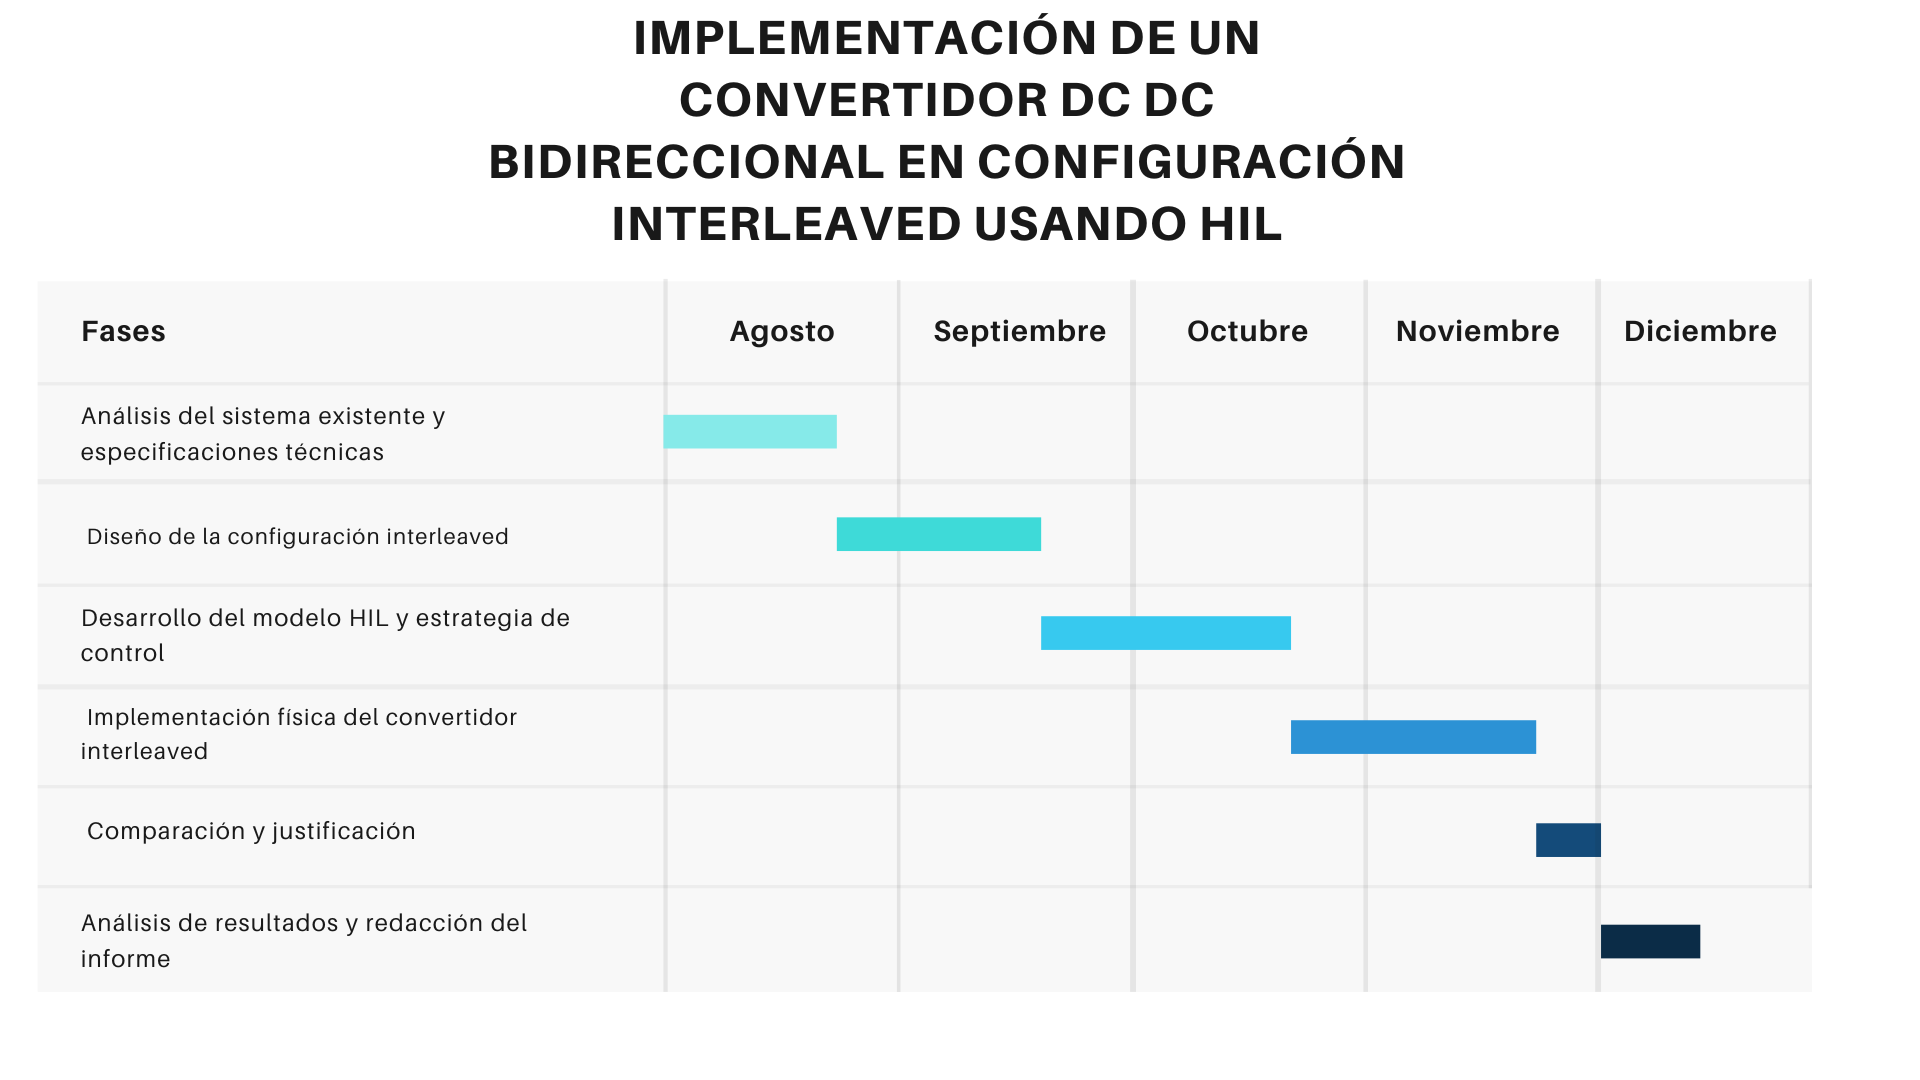
\includegraphics[width=0.9\linewidth]{imgs/Gantt Chart.png}
    \caption{Fases a realizar para el proyecto de grado}
    \label{fig:enter-label}
\end{figure}

\subsection{Identificación y descripción de hitos}


A continuación se describen los hitos clave del proyecto
\renewcommand{\tablename}{Tabla}
\begin{table}[H]
\small % Reduce el tamaño de la letra dentro de la tabla
\begin{tabularx}{\textwidth}{|c| l| X| l|}
\specialrule{1pt}{1pt}{1pt}
\textbf{Nº} & \textbf{Fase} & \textbf{Hito} & \textbf{Fecha estimada} \\
\specialrule{1pt}{1pt}{1pt}
1 & Fase 1 & Inicio del proyecto y levantamiento de información técnica de los módulos físicos existentes. & 4 de agosto de 2025 \\ \hline
2 & Fase 1 & Identificación de parámetros eléctricos (tensión, corriente, frecuencia). & 11 de agosto de 2025 \\ \hline
3 & Fase 2 & Selección de módulos y diseño preliminar de conexión interleaved. & 25 de agosto de 2025 \\ \hline
4 & Fase 2 & Simulación inicial del convertidor interleaved. & 10 de septiembre de 2025 \\ \hline
5 & Fase 3 & Modelado del convertidor interleaved en entorno HIL. & 20 de septiembre de 2025 \\ \hline
6 & Fase 3 & Implementación de control digital y validación HIL. & 10 de octubre de 2025 \\ \hline
7 & Fase 4 & Montaje físico e integración de los módulos en configuración interleaved. & 20 de octubre de 2025 \\ \hline
8 & Fase 4 & Pruebas con cargas reales (baterías y supercondensadores). & 5 de noviembre de 2025 \\ \hline
9 & Fase 5 & Evaluación técnica y comparación con el puente medio tradicional. & 20 de noviembre de 2025 \\ \hline
10 & Fase 6 & Entrega del documento final de tesis. & 10 de diciembre de 2025 \\
\specialrule{1pt}{1pt}{1pt}
\end{tabularx}
\end{table}
